\documentclass{article} % For LaTeX2e
\usepackage{iclr2025_conference,times}
\usepackage[T1]{fontenc}
\usepackage[utf8]{inputenc}
\usepackage{graphicx}
\usepackage{amsmath,amssymb,amsfonts}  % Enhanced math support
\usepackage{booktabs}                   % Better tables
\usepackage{multirow}                   % Multi-row cells in tables
\usepackage{tabularx}                   % Tables with adjustable columns
\usepackage{xcolor}                     % Color support
\usepackage{microtype}                  % Better typography
\usepackage{subcaption}                 % Subfigures and subcaptions
\usepackage{algorithm2e}                % Algorithm formatting
\usepackage{tikz}                       % Drawing and diagrams
\usepackage{wrapfig}                    % Wrap text around figures
\usepackage{makecell}                   % Cell formatting with line breaks

% Optional math commands from https://github.com/goodfeli/dlbook_notation.
\input{math_commands.tex}

\usepackage{hyperref}
\usepackage{url}
\usepackage{cleveref}                   % Better cross-referencing (must be after hyperref)
\usepackage{listings}                   % Code/prompt listings in boxes
\lstset{basicstyle=\ttfamily\small, frame=single, breaklines=true, columns=fullflexible, literate={<}{{\textless}}1 {>}{{\textgreater}}1}

% Define theorem-like environments
\usepackage{amsthm}
\theoremstyle{definition}
\newtheorem{definition}{Definition}[section]


\title{Can Models refuse questions they don't know? \\ Measuring Knowledge-aware Refusal in LLMs}

% Authors must not appear in the submitted version. They should be hidden
% as long as the \iclrfinalcopy macro remains commented out below.
% Non-anonymous submissions will be rejected without review.

\author{Antiquus S.~Hippocampus, Natalia Cerebro \& Amelie P. Amygdale \thanks{ Use footnote for providing further information
about author (webpage, alternative address)---\emph{not} for acknowledging
funding agencies.  Funding acknowledgements go at the end of the paper.} \\
Department of Computer Science\\
Cranberry-Lemon University\\
Pittsburgh, PA 15213, USA \\
\texttt{\{hippo,brain,jen\}@cs.cranberry-lemon.edu} \\
\And
Ji Q. Ren \& Yevgeny LeNet \\
Department of Computational Neuroscience \\
University of the Witwatersrand \\
Joburg, South Africa \\
\texttt{\{robot,net\}@wits.ac.za} \\
\AND
Coauthor \\
Affiliation \\
Address \\
\texttt{email}
}

% The \author macro works with any number of authors. There are two commands
% used to separate the names and addresses of multiple authors: \And and \AND.
%
% Using \And between authors leaves it to \LaTeX{} to determine where to break
% the lines. Using \AND forces a linebreak at that point. So, if \LaTeX{}
% puts 3 of 4 authors names on the first line, and the last on the second
% line, try using \AND instead of \And before the third author name.

\newcommand{\fix}{\marginpar{FIX}}
\newcommand{\new}{\marginpar{NEW}}
\newcommand{\cm}[1]{\textcolor{red}{#1}}
% \newcommand{\cm}[1]{}
\newcommand{\bt}[1]{\textcolor{blue}{#1}}

%\iclrfinalcopy % Uncomment for camera-ready version, but NOT for submission.
\begin{document}


\maketitle

\begin{abstract}
Large Language Models (LLMs) should refuse to answer questions beyond their knowledge, which is a crucial ability for LLMs to be reliable. 
However, existing metrics face three challenges in quantifying this ability: 
\textbf{(1) inaccurate:} yielding inconsistent and biased scores; 
\textbf{(2) complex:} requiring heavy calibration processes; 
and \textbf{(3) indirect:} measuring auxiliary models rather than refusal behavior. 
In this work, we propose a new metric called the \emph{Refusal Index (RI)} to measure how accurately LLMs refuse questions they do not know. 
We define RI as the Spearman's rank correlation between the refusal probability and the error probability. 
To calculate RI, we propose a simple and principled two-pass evaluation that estimates RI from refusal rates in two evaluation runs. 
Experiments across 16 models and 5 datasets show that RI quantifies a model's ability to make accurate knowledge-aware refusals. Unlike existing metrics, RI remains consistent when models exhibit different refusal rates.
RI addresses an important but previously untested aspect of LLM factual evaluation. 
Our observations reveal a blind spot in LLM factual evaluations: 
while LLMs are achieving higher accuracy on factual evaluations, they are not always improving their refusal behavior. 
This finding highlights the need to complement traditional metrics with the Refusal Index for comprehensive factual evaluation.

\end{abstract}

\vspace{-0.7em}
\section{Introduction}
\vspace{-0.7em}
\label{sec:intro}

Large Language Models (LLMs) are increasingly used for knowledge-intensive factual tasks, such as long-term reasoning~\citep{chen2025reasoningerasurveylong} and specialized expert domains~\citep{wang2025capabilitiesgpt5multimodalmedical,gu2024legalagentbench,mahdavi2025brains}. 
Despite these capabilities, LLMs are often poorly calibrated, frequently providing incorrect answers with high confidence~\citep{Huang_2025}. 
An intuitive solution is to enable models to refuse questions beyond their knowledge~\citep{yin2023large}. 
Recent work has explored and strengthened this ability by inducing more accurate refusals with prompting~\citep{cheng2024aiassistantsknowdont, kadavathLanguageModelsMostly2022} or fine-tuning~\citep{zhang2024rtuninginstructinglargelanguage, kapoor2024large}. 
This capability is important for making models more reliable when answering factual questions.

In this paper, we formalize this ability, an LLM's ability to refuse factual questions it does not know, as \emph{knowledge-aware refusal}.
A truly knowledge-aware refusal assesses a model's judgment in two ways: how well a model refuses questions beyond its knowledge (avoiding \emph{overconfidence}) and how well it avoids refusing questions it would answer correctly (avoiding \emph{over-refusal}). 
Traditional factuality metrics fail to capture this property accurately, leaving knowledge-aware refusal insufficiently measured.

\begin{figure}[t]
    \centering
    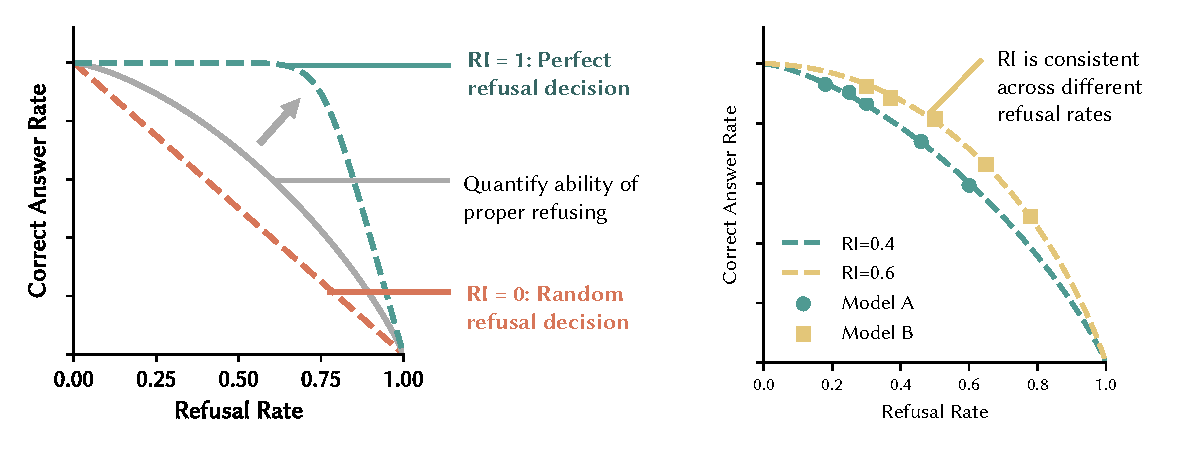
\includegraphics[width=0.95\linewidth]{Figures/RefusalIndex-Illustration.pdf}
    \vspace{-1em}
    \caption{Illustration of Refusal Index (RI). Refusal Index quantifies a model's  internal capability to refuse questions beyond its knowledge by measuring the correlation between refusal decisions and answer incorrectness. Left: Refusal Index models how the correct answer rate drops with increasing refusal rate. Right: Empirical correct answer rates for the same model at different refusal rates align with the Refusal Index. }
    \label{fig:refusal_index_illustration}
    \vspace{-1.5em}
\end{figure}

We propose a metric called the \emph{Refusal Index (RI)} to measure knowledge-aware refusal in factual tasks, which features two key properties:
\textbf{(1) accurate estimates of knowledge-aware refusal}: We formally define the Refusal Index as the Spearman correlation between refusal probabilities and error probabilities (\Secref{sec:refusal_index_method}). 
This definition is independent of refusal rate and directly targets refusal behavior, making it an unbiased measure. 
\textbf{(2) lightweight evaluation procedure}: 
Unlike previous calibration metrics that require expensive calibration processes, we only need two standard evaluation passes to compute RI, which is compatible with existing evaluation pipelines.
Specifically, we first evaluate a model on a factual question-answering dataset, collecting correct answer rates and refusal rates. 
Then, we run a second evaluation pass to regenerate answers for refused questions. 
Finally, we compute RI using the correct answer rates and refusal rates from both evaluation passes.

We perform extensive experiments and analyses to validate RI across 16 models on 5 datasets. 
We demonstrate that RI quantifies models' capability to refuse questions they do not know. 
As shown in \Figref{fig:refusal_index_illustration}, RI parameterizes the relationship between correct answer rates and refusal rates through an accuracy-refusal curve, whose convexity captures a model's ability to minimize false refusals.
This analytical model is supported by the empirical results, with consistent RI scores on the same model at different refusal rates, which align with the accuracy-refusal curve.
We also discover that RI has high agreement with established calibration metrics and provides consistent model rankings independent of a model's correctness and refusal rates. 

Beyond RI's efficacy in capturing knowledge-aware refusal, we leverage it to reveal a critical gap in current factuality evaluation: the disconnect between factual accuracy and knowledge-aware refusal capabilities. Our analysis reveals three key insights that traditional metrics overlook:
\textbf{(1) RI identifies persistent capability gaps.} While LLMs achieve high accuracy on factual tasks, their refusal behavior is unreliable. This gap remains stable across different prompting strategies and cannot be resolved by simply improving accuracy or adjusting refusal rates;
\textbf{(2) Training data and pipelines influence refusal behavior.} The model family emerges as the strongest predictor of knowledge-aware refusal ability, with certain families consistently outperforming others regardless of model scale; and
\textbf{(3) Knowledge-aware refusal is sensitive to noisy context.} Models exhibit significantly degraded refusal performance when ground truth information is unavailable in the provided context, suggesting over-reliance on contextual cues.
These findings demonstrate that RI captures an essential dimension of model reliability absent from existing factuality metrics, highlighting the need to incorporate knowledge-aware refusal measures for a more comprehensive factuality evaluation.


\vspace{-0.7em}
\section{Refusal Index}
\vspace{-0.7em}
\label{sec:refusal_index_method}

% We begin by defining the scope and objective of our research. When evaluating calibration, we want to measure whether, higher confidence in model answers leads to a higher accuracy. More precisely, whether the model's output probability aligns with the actual probability of being correct. However, evaluating either probability or correctness for arbitrary text outputs remains an open problem, as ground truth can be subjective, non-deterministic, or unavailable.

% \noindent\textbf{Problem.}
% Measuring an LLM's ability to refuse questions beyond its knowledge presents several challenges.
% On the one hand, refusal decisions are not solely determined by a model's self-knowledge. 
% Instead, model preferences, question risk levels, or explicit instructions can influence these decisions. 
% Consequently, these factors preclude simply counting refusal rates to evaluate knowledge-aware refusal. 
% For example, a model designed with a higher refusal tendency will easily achieve a higher score when measured with refusal rate on unanswerable questions, regardless of its actual knowledge.
% On the other hand, we cannot rely on external calibrators like verbalized confidence~\citep{xiong2023can} or linear probe to replace direct refusal measurements, because these calibrators may not accurately reflect a model's internal self-knowledge about when to refuse.
% Therefore, an effective metric for knowledge-aware refusal must: (1) quantify knowledge-aware refusal accurately, (2) remain consistent across different refusal rates, and (3) derive directly from black-box LLM outputs.

\noindent\textbf{Scope.} 
Our evaluation settings follow widely used factuality evaluations like SimpleQA and TruthfulQA~\citep{wei2024measuringshortformfactualitylarge, lin2022truthfulqameasuringmodelsmimic}, where models provide atomic answers for short-form, factual questions. 
Additionally, models can refuse to answer to avoid hallucination by producing outputs such as \emph{``I don't have enough information...''}.
Following SimpleQA, each model answer is classified as correct, incorrect, or refused by comparing it against the ground truth. 
The classification results are used to estimate the model's factuality level, or in our case, the ability to make knowledge-aware refusals.
This formulation avoids subjective grading and partial correctness in LLM generation, allowing more reliable measurement.

\noindent\textbf{Notations.}
Formally, we denote the LLM as $f_{\text{LM}}: \mathcal{X} \rightarrow \mathcal{Y} \cup \{\bot\}$, where $x \in \mathcal{X}$ represents the input question, $y \in \mathcal{Y}$ represents the output answer, and $\bot$ denotes refusal. 
For the $i$-th question $x_i$ with ground truth $y_i$ in dataset $D$, we define two indicators: $W_i = \mathbf{1}\{f_{\text{LM}}(x_i) \neq y_i\}$ for incorrect outputs (including refusals) and $R_i = \mathbf{1}\{f_{\text{LM}}(x_i) = \bot\}$ for refusal responses. 
We define the error probability $w_i = P(f_{\text{LM}}(x_i) \neq y_i)$ and the refusal probability $r_i = P(f_{\text{LM}}(x_i) = \bot)$. 
Conceptually, a model with better knowledge-aware refusal should refuse more frequently as questions become more difficult. 
We measure this ability with the \emph{Refusal Index}. 
Inspired by rank-based calibration metrics like AUROC~\citep{NiculescuMizil2005PredictingGP}, we define the Refusal Index as the correlation between refusal probabilities and error probabilities:

\begin{definition}[Refusal Index]
Refusal Index $\rho_S$ is defined as Spearman's rank correlation between the model's refusal probability $r_i$ and the error probability $w_i$ as follows:

\vspace{-1em}
\begin{equation}
   \text{Refusal Index} = \rho_S  = \text{Corr}(\text{Rank}(r_i), \text{Rank}(w_i)).
\end{equation}
\vspace{-1.5em}

\end{definition}

The intuition behind the definition is that a model achieves \emph{perfect knowledge-awareness} when its refusal probability increases monotonically with error probability, making it more likely to refuse as questions become more difficult:

\vspace{-1em}
\begin{equation}
w_i \leq w_j \iff P(f_{\text{LM}}(x_i) = \bot) \leq P(f_{\text{LM}}(x_j) = \bot).
\label{eq:refusal_perfect_calibrated}
\end{equation}
\vspace{-1.5em}

Note that this differs from error-based calibration metrics like Expected Calibration Error (ECE), which quantify absolute discrepancies between $r_i$ and $w_i$. 
In contrast, our approach evaluates only the rank discrepancies between $r_i$ and $w_i$.
We define RI as a discrimination property because it captures the fundamental aspect of knowledge-aware refusal. 
This is because absolute discrepancy-based metrics are sensitive to changes in a model's overall refusal rate, which can significantly affect the metric value (an undesirable property). 
In contrast, discriminative metrics like RI or AUROC measure only the rank between different samples, making them more robust to changes in overall refusal rates. 
Alternatively, it is generally easier for a model to adjust its overall refusal rate than to improve its ability to rank questions by difficulty accurately.
Next, we introduce how to estimate the Refusal Index through a two-pass evaluation process (\Secref{sec:two_pass_evaluation}).


\vspace{-0.5em}
\subsection{Two-Pass Evaluation}
\vspace{-0.5em}
\label{sec:two_pass_evaluation}

The naive way to measure RI would require the refusal probability $P(f_{\text{LM}}(x_i) = \bot)$ across questions with varying error probabilities. 
However, in factuality evaluation, we only observe single text output from the model, making refusal probabilities inaccessible. 
To address this issue, we propose a two-pass evaluation process to infer the Spearman correlation between refusal and error probabilities from binary observations. 
This approach models refusal decisions by first treating refusal and correctness indicators as results of thresholding on their respective probabilities, and then modeling their joint distribution with a Gaussian copula. 


\noindent\textbf{Formulating the Joint Distribution.} We estimate $\rho_S$ from the joint distribution of refusal and error probabilities using a Gaussian copula model with correlation $\rho$ as follows:

\vspace{-1em}
\begin{equation}
C(u,v) = \Phi_\rho\!\big(\Phi^{-1}(u), \Phi^{-1}(v)\big).
\end{equation}
\vspace{-1.5em}

Here, $u = F_r(r_i)$ and $v = F_e(w_i)$ are the marginal CDFs, $\Phi^{-1}$ is the standard normal quantile function, and $\Phi_\rho$ is the bivariate standard normal CDF with correlation $\rho$. 
This Gaussian copula specifies only the dependence on $\rho$ and leaves the marginal distributions of $r_i$ and $w_i$ unrestricted. 
The function $\Phi_\rho$ depends only on rank correlation, remaining independent of the marginal distributions. 
Next, we avoid modeling $F_r$ and $F_e$ directly and instead estimate $\rho$ from $R_i$ and $W_i$ via maximum likelihood. 
We then compute $\rho_S$ from $\rho$ using the standard conversion formula for Gaussian copulas: $\rho_S = \frac{6}{\pi}\arcsin\!\left(\frac{\rho}{2}\right)$~\citep{kendall1979advanced}. 
Because $\rho$ determines the corresponding rank correlations of $r_i$ and $w_i$ via a monotonic transformation, we could equivalently report other rank measures such as Kendall's $\tau$ instead of $\rho_S$. We use Spearman's $\rho$ for interpretability.

\begin{wrapfigure}{r}{0.5\textwidth}
    \vspace{-1em}
    \centering
    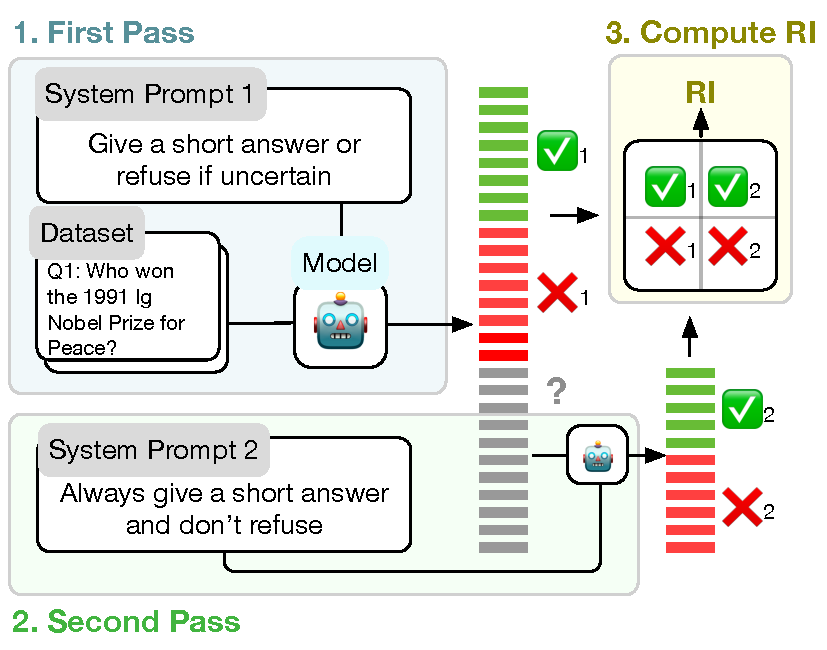
\includegraphics[width=0.45\textwidth]{Figures/two-pass.pdf}
    \caption{Illustration of two-pass evaluation process.}
    \label{fig:two_pass_evaluation}
    \vspace{-1.5em}
\end{wrapfigure}

Estimating $\rho$ requires observing two binary indicators for each sample: $R_i$ for refusal probability $r_i$ and $W_i$ for error probability $w_i$, while $r_i$ and $w_i$ themselves remain latent. 
We achieve this through a two-pass evaluation that runs the model on the same dataset twice. 
The first pass observes refusal decisions $R_i$, using a standard setup that allows the model to answer or refuse each question, classifying responses as correct, incorrect, or refused. 
The second pass observes correctness $W_i$ by updating the system prompt to remove abstention options and requiring the model to answer all questions. We provide prompt details in \Secref{app:system_prompts} and an illustration in \Figref{fig:two_pass_evaluation}.
We run the second pass only on questions refused in the first pass, collecting correctness indicators $W'_i$ for all refused questions ($R_i = 1$).

\noindent\textbf{Estimating Refusal Index.} We define the aggregated correctness indicator $\hat{W}_i = R_i \cdot W'_i + (1-R_i) \cdot W_i$ as the correctness when the model provided an answer. 
The empirical refusal rate is $r=\sum_{i=1}^{|D|} R_i/|D|$ and the error rate is $\mu = \sum_{i=1}^{|D|} \hat{W}_i/|D|$. 
Under our model, the pair $(R,\hat{W})$ results from thresholding a bivariate standard normal vector $(Z_R,Z_W)$ with correlation $\rho$ at, matching the standard tetrachoric setup implied by the copula.


\vspace{-1em}
\begin{equation}
    \begin{aligned}
        \tau_R=\Phi^{-1}(1-r), \qquad \tau_W=\Phi^{-1}(1-\mu).
    \end{aligned}
\end{equation}
\vspace{-1.5em}

Let $n_{ab}$ be the counts of $(R=a, \hat{W}=b)$ for $a,b\in\{0,1\}$. The cell probabilities are

\vspace{-1em}
\begin{equation}
    \begin{aligned}
    p_{11}(\rho) &= \bar\Phi_2\!\big(\tau_R,\tau_W;\rho\big) \;=\; P(Z_R>\tau_R, Z_W>\tau_W),\\
    p_{10}(\rho) &= r - p_{11}(\rho),\qquad
    p_{01}(\rho) \;=\; \mu - p_{11}(\rho),\\
    p_{00}(\rho) &= 1 - r - \mu + p_{11}(\rho).
    \end{aligned}
\end{equation}
\vspace{-1em}

We estimate $\hat\rho$ by maximizing the multinomial log-likelihood and use $\hat\rho$ to compute $\rho_S$:

\vspace{-1em}
\begin{equation}
    \begin{aligned}
        \hat\rho = \argmax_{\rho \in (-1,1)} \ell(\rho), \quad \text{where} \quad \ell(\rho) = \sum_{a,b\in\{0,1\}} n_{ab} \log p_{ab}(\rho).
        \label{eq:ri-estimation}
    \end{aligned}
\end{equation}
% \vspace{-1.5em}


\vspace{-0.7em}
\section{Experiments \& Results}
\vspace{-0.5em}
\label{sec:experiments}

% \vspace{-0.5em}
\subsection{Experimental Setup}
\vspace{-0.5em}
\label{sec:experimental_setup}

\noindent\textbf{Models.} We evaluate RI on 16 models across different families, sizes, and architectures to ensure comprehensive coverage. 
Our open-source models include \emph{Gemma-3-12B}~\citep{gemma3_2025}, \emph{Qwen3-32B/235B}~\citep{qwen3_2025} in both think and no-think modes, \emph{Qwen2.5-72B-Instruct}~\citep{qwen2_5_2024}, \emph{Llama 3.1 70B} \citep{llama3_2024}, \emph{Mistral-Large-Instruct-2411}~\citep{mistral_large_2_2024}, \emph{GLM-4.5 and GLM-4.5-Air}\citep{glm45_2025} and \emph{DeepSeek-V3-0324}~\citep{deepseek_v3_2024}. 
Our proprietary models include \emph{Claude 3.5 haiku} \citep{claude35_2024}, \emph{Claude Sonnet 4} \citep{claude4_2025}, \emph{GPT4.1} and \emph{GPT4.1 mini} \citep{gpt41_2025} and \emph{Gemini 2.5 Flash} and \emph{Gemini 2.5 Flash Lite} \citep{gemini25_2025}. 
We use temperature=0.7 and top-p=0.95 across all models. 
More implementation details are provided in \Secref{sec:detailed_experimental_setup}.

\noindent\textbf{Datasets.} We evaluate RI on three scenarios that require model to make accurate, knowledge-aware refusals: factual question answering, extrinsic hallucination detection (hallucination from training data), and intrinsic hallucination detection (hallucination from context).
(1) We use factual question answering to test models' ability to refuse unknown facts. 
Specifically, we use SimpleQA \citep{wei2024measuringshortformfactualitylarge}, which contains verifiable, atomic factual questions that challenge even frontier LLMs. 
(2) We use extrinsic hallucination detection to test whether models correctly refuse to answer when they cannot recall knowledge from training data. 
For this scenario, we use PreciseWikiQA \citep{bangHalluLensLLMHallucination2025}, a dynamically generated question-answering dataset from Wikipedia snippets. 
PreciseWikiQA tests whether models hallucinate information from their training data, assuming Wikipedia knowledge was included during training. 
We follow \citet{bangHalluLensLLMHallucination2025} to generate 2000 questions for evaluation. 
(3) We use intrinsic hallucination detection to test whether models can faithfully recall information with noisy context. 
For this scenario, we use the 3 datasets from FaithEval \citep{ming2025faithevallanguagemodelstay}. 
However, because the \texttt{Unanswerable} and \texttt{Inconsistency} subsets lack ground truth required for RI computation, we create a 1:1 mixed dataset of PreciseWikiQA and FaithEval to report RI.

\noindent\textbf{Baseline Metrics.} We compare RI against five established metrics for measuring knowledge-aware refusal (Table~\ref{tab:baseline_metrics}): Correct Answer Rate, Refusal Rate, Correct given Attempted (C/A), F-score, and Weighted Score. 
We pick $p=0.2$ for the Weighted Score to balance the accuracy and refusal rate. 
We classify all model outputs into three categories following SimpleQA: (1) Correct, (2) Incorrect, or (3) Not Attempted (refusal).




\noindent\textbf{Adjusting Refusal Rates.} We test RI's consistency by measuring how it changes when models exhibit different refusal rates. 
To this end, we use different system prompts to instruct models to be more conservative or active in answering questions. 
These prompts modify refusal tendencies without degrading the quality of refusal decisions, as shown in \Secref{sec:prompt_design_evaluation}.
Specifically, we use four different system prompts to evaluate each model with varying refusal rates in the first pass, while keep one default prompt that instructs models to answer all questions in the second pass. 
The complete system prompts are provided in \Secref{app:system_prompts}.


\subsection{Refusal Rate Stability Analysis}
\label{sec:refusal_index_validation}


\begin{table*}[t]
    \centering
    \small
    \caption{Score stability across different refusal rates. We run evaluation with different refusal tendencies on SimpleQA for each model. $\Delta_{\text{Metric}}$ denotes the normalized difference between most-refusal and least-refusal runs. We use $p=0.2$ for the Weighted metric. Lower is better.}
    \label{tab:qwen25_simpleqa_prompt_strategies}
    \begin{tabularx}{\textwidth}{>{\raggedright\arraybackslash}p{0.12\textwidth} >{\raggedright\arraybackslash}p{0.15\textwidth} *{6}{>{\centering\arraybackslash}X}}
        \toprule
        \textbf{Type} & \textbf{Model} & \textbf{$\Delta_{\text{Accuracy}}$} & \textbf{$\Delta_{\text{Refusal}}$} & \textbf{$\Delta_{\text{C/A}}$} & \textbf{$\Delta_{\text{F-score}}$} & \textbf{$\Delta_{\text{Weighted}}$} & \textbf{$\Delta_{\text{RI}}$} \\
        \midrule
        \multirow{5}{*}{\makecell{Normalized \\ Difference}} & Mistral-123B & $-0.40$ & $+0.93$ & $+0.37$ & $-0.16$ & $-0.83$ & $\mathbf{+0.06}$ \\
         & Qwen2-35B & $-0.47$ & $+0.95$ & $+0.12$ & $-0.31$ & $-0.62$ & $\mathbf{-0.19}$ \\
         & Qwen2.5-72B & $-0.84$ & $+0.43$ & $+0.50$ & $-0.60$ & $-1.32$ & $\mathbf{-0.07}$ \\
         & Qwen3-32B & $-0.96$ & $+0.54$ & $+0.48$ & $-0.71$ & $-1.42$ & $\mathbf{+0.14}$ \\
         & Average & $-0.73$ & $+0.72$ & $+0.50$ & $-0.50$ & $-1.17$ & $\mathbf{+0.08}$ \\
        \midrule
         & \textbf{Model} & \textbf{$CV_{\text{Accuracy}}$} & \textbf{$CV_{\text{Refusal}}$} & \textbf{$CV_{\text{C/A}}$} & \textbf{$CV_{\text{F-score}}$} & \textbf{$CV_{\text{Weighted}}$} & \textbf{$CV_{\text{RI}}$} \\
        \midrule
        \multirow{5}{*}{\makecell{Coefficient of \\ Variation}} & Mistral-123B & $0.16$ & $0.35$ & $0.14$ & $0.06$ & $0.31$ & $\mathbf{0.04}$ \\
         & Qwen2-35B & $0.22$ & $0.47$ & $0.06$ & $0.14$ & $0.32$ & $\mathbf{0.09}$ \\
         & Qwen2.5-72B & $0.35$ & $0.17$ & $0.19$ & $0.26$ & $0.53$ & $\mathbf{0.03}$ \\
         & Qwen3-32B & $0.35$ & $0.19$ & $0.17$ & $0.28$ & $0.51$ & $\mathbf{0.07}$ \\
         & Average & $0.29$ & $0.29$ & $0.19$ & $0.21$ & $0.46$ & $\mathbf{0.08}$ \\
        \bottomrule
    \end{tabularx}
\end{table*}


In this section, we validate the Refusal Index and analyze its stability across different refusal rates. 
We demonstrate that: (1) the Refusal Index conceptualizes and evaluates the model's knowledge-aware refusal with an \emph{accuracy-refusal curve}, and (2) the two-pass evaluation returns consistent RI across different refusal rates.

\paragraph{RI Measures Knowledge-aware Refusal with Accuracy-Refusal Curve}
An accuracy-refusal curve measures knowledge-aware refusal by showing the correct answer rate at each refusal rate for a model on the same dataset.
While refusing more uncertain questions reduces incorrect answers, it also leads to fewer correct answers due to false refusals. 
By varying the overall refusal rate, each model exhibits a trade-off between correct answers and refusal rate. 
As shown in Figure~\ref{fig:acc_rej_plot_with_contour_lines}, fixing any metric constant gives a unique iso-score curve in the accuracy–refusal plane, which describes the accuracy-refusal trade-off relationship assumed by the metric.

\begin{wrapfigure}{r}{0.48\textwidth}
    \centering
    \vspace{-1.5em}
    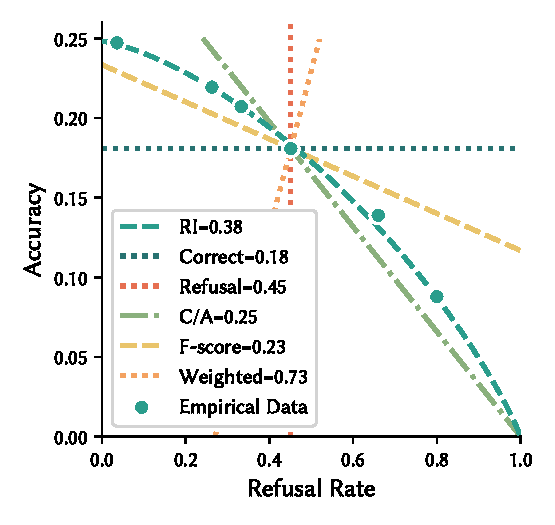
\includegraphics[width=0.48\textwidth]{Figures/acc_rej_plot_with_contour_lines.pdf}
    \caption{Comparison of factuality metrics with iso-score accuracy-refusal trade-off curves. C/A, F, and W correspond to Correct / Attempted, F-score, and Weighted score, respectively.}
    \vspace{-1em}
    \label{fig:acc_rej_plot_with_contour_lines}
\end{wrapfigure}


Compared with heuristic metrics, iso-RI curves have two desirable properties: (1) they represent sensible accuracy–refusal trade-offs matching the expected behavior of the model (see Figure~\ref{fig:refusal_index_illustration}, left). 
Different iso-RI curves yield the same maximum correct answer number when the refusal rate is 0 and reach zero correct answers when the refusal rate is 1; and (2) RI is agnostic to the maximum correct answer number and refusal rate, controlling only the convexity of the curve and capturing how well a model preserves correct answers by reducing false refusals. 
That is, for two models with the same maximum correct answer number, the one with higher RI retains more correct answers when refusing the same fraction of questions. 
In contrast, heuristic metrics fail to capture this property, imposing approximately linear accuracy–refusal relationships at fixed scores. 
In summary, the Refusal Index does not simply reward higher correct answer rate or lower refusal rates, but captures the level of rank calibration in refusal decisions, distinct from all previous metrics.

% \begin{figure}[t]
%     \centering
%     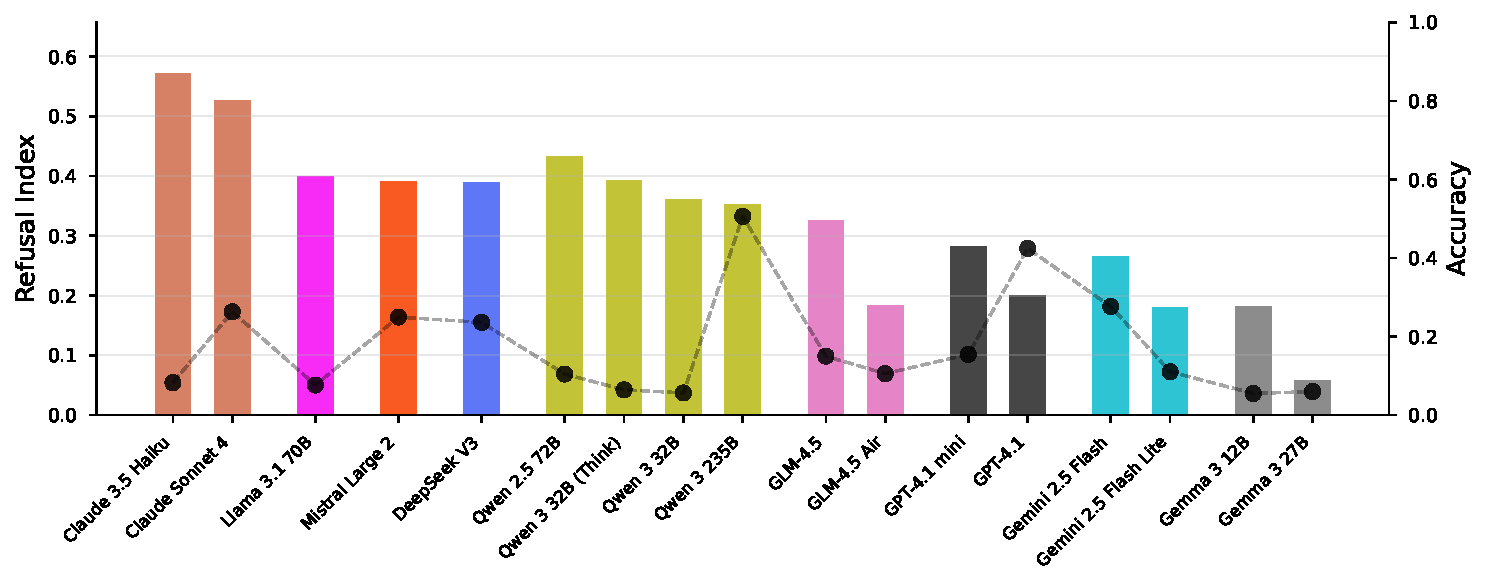
\includegraphics[width=0.95\linewidth]{Figures/simpleqa_refusal_index.pdf}
%     \caption{Evaluation results of the Refusal Index on SimpleQA. }
%     \label{fig:simpleqa_refusal_index}
% \end{figure}

\paragraph{RI remains consistent across different refusal rates.}
To empirically validate RI, we test whether the Refusal Index remains consistent across different refusal rates. 
For this, we design a set of system prompts that progressively encourage caution in answering to induce different refusal rates, then apply them to the same model on the SimpleQA dataset. 
Our results demonstrate that RI exhibits remarkable stability across these different refusal rates, while heuristic metrics show substantial variation. 
As shown in Table~\ref{tab:qwen25_simpleqa_prompt_strategies}, RI exhibits approximately 70\% lower variability compared to heuristic metrics. 
This empirical finding suggests that prompt-induced changes in refusal rate shift the refusal probability distribution without changing the correlation between refusal probability and error probability. 
In the appendix, we provide additional validation through goodness-of-fit tests for the Gaussian copula assumption.


\subsection{Alignment with Calibration Methods}

\paragraph{RI is highly consistent with sampling-based calibration methods.}
One potential concern with RI is that although it is defined as the rank correlation between refusal probability and error probability, the two-pass evaluation may not faithfully reflect that correlation. 
To address this, we compare RI values with AUROC scores computed using P(Answering) as an uncertainty estimation method. 
We choose AUROC with P(Answering) for a fair comparison because it shares the same definition of uncertainty as RI. 
Specifically, (1) AUROC is a rank-calibration metric that only measures the discriminative ability of refusal and (2) P(Answering) is a direct estimation of the prediction probability for model refusals. 
While there exist other calibration metrics like ECE, Brier Score, and various uncertainty estimation methods, AUROC with P(Answering) is the most direct measurement of the correlation between refusal and error.
\Figref{fig:comparison_auroc} shows the results. 
Among the evaluated metrics, RI demonstrates the strongest positive correlation with AUROC at 85\%, outperforming all other metrics.
This high agreement between RI and AUROC with P(Answering) suggests that RI accurately reflects the correlation between refusal probability and error probability.
Meanwhile, RI requires much smaller computational overhead compared to estimating P(Answering) with multiple sampling.


\begin{figure}[t]
    \centering
    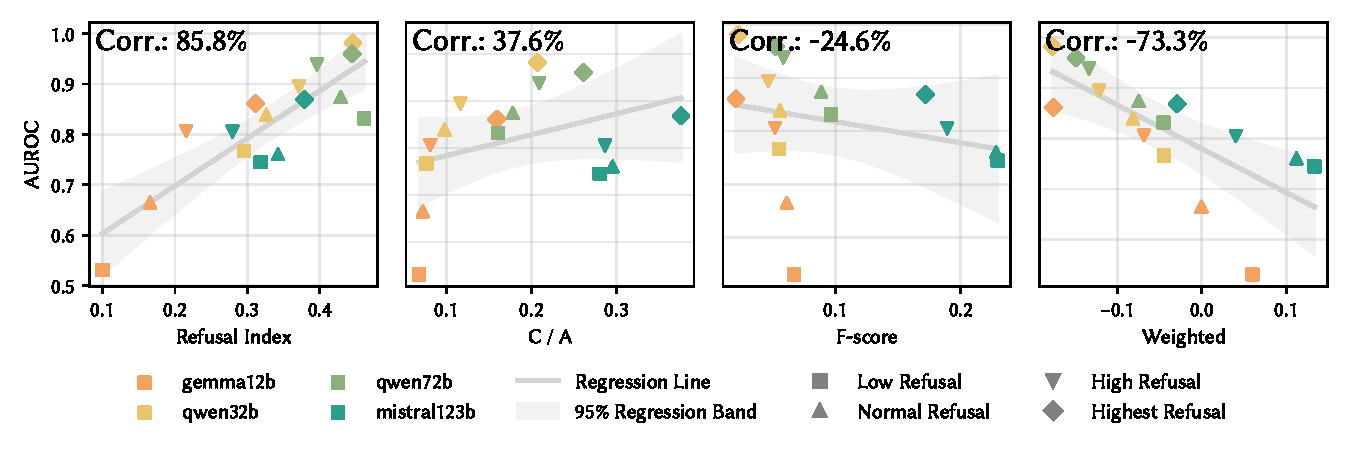
\includegraphics[width=\linewidth]{Figures/comparison_auroc_panswer.pdf}
    \caption{Correlation between factuality metrics and AUROC with P(Answering) on SimpleQA. RI shows the highest positive correlation with AUROC while being orders of magnitude cheaper to compute.}
    \label{fig:comparison_auroc}
\end{figure}

\subsection{Model Ranking Stability}

Finally, we study whether the knowledge-aware refusal measured by RI is consistent across different models and datasets. 
To this end, we measure model ranking stability: does RI rank models consistently in different datasets or evaluation settings? 
Higher ranking stability suggests that a metric captures genuine, discriminative properties of models. 
Specifically, we calculate Kendall's $W$ (overall ranking agreement) and Winner Entropy (top-1 consistency) on all 8 evaluation settings (4 refusal-varying evaluations on SimpleQA + 4 hallucination benchmarks). 
Additionally, to capture the ranking stability of the correlation structure between correct answers and refusals, we want to filter out the sole effect from the correct answer rate or refusal rate. 
We make the removal by performing an isotonic regression on the correct answer rate or refusal rate across different setups for each model, then remove the regressed values from each metric. We calculate the Kendall's $W$ and Winner Entropy on the residuals, effectively measuring parts of the metric that cannot be explained by correct answer rate or refusal rate alone.

\paragraph{RI provides stable model rankings independent of accuracy and refusal rate.} 
As shown in Table~\ref{tab:ranking_stability}, when removing the monotonic effect of correct answer rate or refusal rate, RI still shows high ranking stability, while heuristic metrics degrade to near random values. 
We can see that heuristic metrics like F-score and Weighted achieve very good ranking stability, but their Kendall's $W$ and Winner Entropy drop quickly when we remove the monotonic effect from correct answer rate or refusal rate. 
This result suggests that while heuristic metrics like F-score have high ranking stability, they are mostly explained by correct answer rate or refusal rate. 
In contrast, RI retains most of its ranking stability even after removing the effects from correct answer rate and refusal rate, indicating that it captures the intrinsic knowledge-aware refusal of models, persisting across different evaluation settings.


\begin{table}[t]
    \centering
    \small
    \caption{Ranking stability across different evaluation settings. $-\text{Correct}$ and $-\text{Refusal}$ show results after removing monotonic effects of correct answer rate and refusal rate with isotonic regression. $- \text{Both}$ removes both correctness and refusal rates with additive isotonic regression.}
    \label{tab:ranking_stability}
    \setlength{\tabcolsep}{4pt}
    \begin{tabular}{lcccccccc}
        \toprule
         & \multicolumn{4}{c}{\textbf{Kendall's W} $\uparrow$} & \multicolumn{4}{c}{\textbf{Winner Entropy} $\downarrow$} \\
        \cmidrule(lr){2-5} \cmidrule(lr){6-9}
        \textbf{Metric} & \textbf{Default} & \textbf{$- \text{Correct}$} & \textbf{$- \text{Refusal}$} & \textbf{$- \text{Both}$} & \textbf{Default} & \textbf{$- \text{Correct}$} & \textbf{$- \text{Refusal}$} & \textbf{$- \text{Both}$} \\
        \midrule
        Random Value  & 0.25 & 0.25 & 0.25 & 0.25 & 0.61 & 0.61 & 0.61 & 0.61 \\
        Correct Answer Rate & 0.87 & 0.00 & \textbf{0.48} & 0.39 & \textbf{0.00} & 1.00 & 0.48 & 1.00 \\
        Refusal Rate & 0.86 & 0.44 & 0.00 & 0.30 & 0.18 & 0.61 & 1.00 & 1.00 \\
        \midrule
        C / A    & 0.69 & \textbf{0.63} & 0.40 & 0.37 & 0.33 & 0.61 & 0.48 & 0.61 \\
        F-score  & \textbf{0.90} & 0.10 & 0.48 & 0.39 & 0.00 & \textbf{0.18} & 0.48 & 0.52 \\
        Weighted & 0.87 & 0.60 & 0.25 & 0.32 & 0.33 & 0.33 & \textbf{0.37} & 0.61 \\
        RI       & 0.47 & 0.50 & 0.35 & \textbf{0.49} & 0.47 & 0.33 & 0.61 & \textbf{0.37} \\
        \bottomrule
    \end{tabular}%
    \\
\end{table}

\section{Discussion}
\label{sec:discussion}

In the previous section, we have validated the Refusal Index with its analytical model and experimental results, showing that the RI uniquely and consistently evaluates the knowledge-aware refusal ability. 
In this section, we provide insights into LLM factuality through the lens of Refusal Index. 
Our interpretable and practical method provides several new insights into model calibration that were previously obscured by heuristic metrics. 



\paragraph{Does prompting models to be more cautious mitigate miscalibration?} LLMs are notorious for their overconfidence; by default, LLMs will try to answer all questions beyond their knowledge. 
One might wonder whether instructing models to reduce confidence helps with this problem. 
Our proposed RI gives a more holistic understanding to this question. 
As shown in Table~\ref{tab:qwen25_simpleqa_prompt_strategies}, while increasing refusal rates increases the correct answer rate in answered questions (increasing C/A), their RI remains stable and far from perfection. 
This means that even when a model shows the same refusal rate as its error rate (no system bias), there still remains a gap from perfect refusal decisions (perfect alignment between refusal and error). 
In other words, RI indicates and quantifies this gap independent of specific refusal rates from the model.

\paragraph{What factors lead to better knowledge-aware refusal?}

\begin{wrapfigure}{r}{0.5\textwidth}
    \centering
    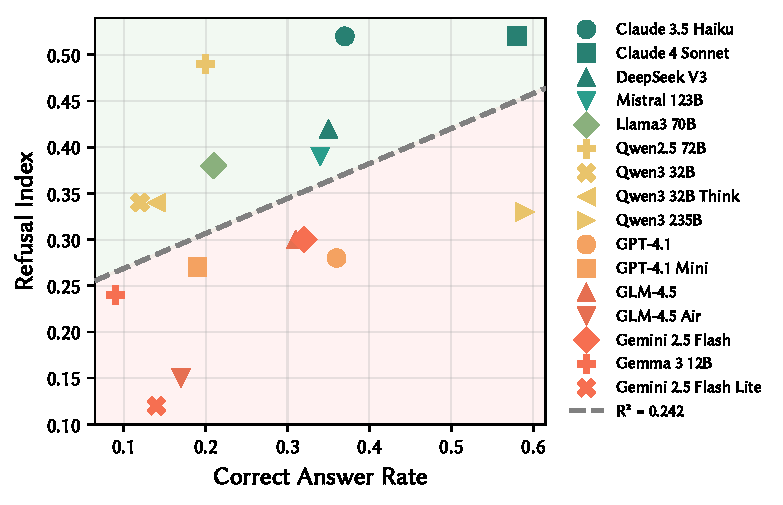
\includegraphics[width=0.45\textwidth]{Figures/simpleqa_refusal_vs_accuracy_scatter.pdf}
    \caption{Scatter plot of Refusal Index vs. Correct Answer Rate.}
    \label{fig:simpleqa_refusal_vs_accuracy_scatter}
\end{wrapfigure}

Naturally, we are curious about what factors in LLM designs have the most impact on RI. 
Within the model scope covered in our test, we didn't find high correlation between RI and model parameter sizes, accuracy, or refusal rates. 
We plot the relationship between correct answer rate in SimpleQA under normal refusal rates and their average RI, as shown in the scatter plot in \Figref{fig:simpleqa_refusal_vs_accuracy_scatter}. 
The correct answer rate shows a mere $R^2=0.235$ correlation to Refusal Index, suggesting higher model accuracy at factual tasks does not necessarily lead to more knowledge-aware refusals. 
Interestingly, we find \emph{model family} is a strong predictor of RI. 
In our experiments, models from \emph{Claude} and \emph{Qwen} (except Qwen 235B) are well above the regression line, showing above-average knowledge-aware refusal abilities. 
In contrast, all models from \emph{Gemini}, \emph{GPT-4.1} and \emph{GLM-4.5} are below the regression line. 
Especially \emph{Claude} models show the highest RI on both Claude-3.5 Haiku and Claude-3.5 Sonnet. 
These findings hint that the specific training pipeline and data distribution used by different model providers might play a more important role in the knowledge-aware refusals.

\begin{wraptable}{r}{0.6\textwidth}
    \vspace{-\baselineskip}
    \centering
    \caption{Refusal Index results on hallucination benchmarks.}
    \label{tab:hallu_model_comparison}
    \resizebox{\linewidth}{!}{%
    \begin{tabular}{l c c c c}
    \toprule
    \multirow{3}{*}{\textbf{Model}} & \multicolumn{2}{c}{\textbf{Truth Available}} & \multicolumn{2}{c}{\textbf{Truth Unavailable}} \\
    \cmidrule(lr){2-3} \cmidrule(lr){4-5}
    & \textbf{Precise-} & \textbf{Counter-} & \textbf{Incon-} & \textbf{Unans-} \\
    & \textbf{Wiki} & \textbf{factual} & \textbf{sistency} & \textbf{werable} \\
    \midrule
    Gemma-3-12b & 0.36 & 0.56 & 0.22 & 0.12 \\
    Qwen3-32B & 0.48 & 0.60 & 0.27 & 0.24 \\
    Qwen2.5-72B & \textbf{0.54} & 0.56 & 0.22 & 0.40 \\
    Llama-3.1-70B & 0.52 & \textbf{0.70} & 0.17 & 0.31 \\
    Mistral-Large & 0.50 & 0.38 & \textbf{0.34} & \textbf{0.52} \\
    \midrule
    Average & 0.48 & 0.56 & 0.24 & 0.32 \\
    \bottomrule
    \end{tabular}%
    }
    \vspace{-0.5em}

\end{wraptable}

\paragraph{Is a model's refusal ability affected by context?} 
We further expand RI to a more realistic setting where models generate answers conditioned on grounding context. 
In Table~\ref{tab:hallu_model_comparison}, each dataset tests model refusal ability in different scenarios:
\textbf{PreciseWiki} requires models to recall information from training data; 
\textbf{Counterfactual} tests models' ability to refrain from hallucinating from misleading and counterfactual context (e.g., the moon is made of cheese). 
\textbf{Inconsistency} and \textbf{Unanswerable} test if models refuse when answers are not available, where \textbf{Inconsistency} provides conflicting information and \textbf{Unanswerable} does not provide answers in context.
Results show that RI values for PreciseWiki are similar to those of SimpleQA, and models generally have good ability to identify and avoid counterfactual context. However, when ground truth becomes unavailable, models are showing much worse knowledge-aware refusal. 
This suggests that models' knowledge-aware refusal may rely on existing partial information on the answer; they make poorer knowledge-aware refusals when the answer never appears in training data or context.

\paragraph{Limitations of RI.}
While the Refusal Index is a useful metric for measuring knowledge-aware refusal, there are limitations that practitioners should be aware of. 
First, as the two-pass evaluation requires instructing the model to either refuse or provide forced answers, it requires a relatively capable model. 
Second, our formulation and validation of RI are focused on \emph{knowledge-aware refusal}, which may not hold for other kinds of refusals, such as refusals for safety reasons. 
Finally, from both the definition and experimental results, knowledge-aware refusal is a relatively weak signal compared to other metrics like correct answer rate. 
Thus, we recommend using larger datasets in evaluation to obtain a more stable RI score. 
Nevertheless, RI provides a pragmatic metric for knowledge-aware refusal, which is important but overlooked by previous metrics.

\vspace{-0.7em}
\section{Related Work}
\vspace{-0.7em}
\label{sec:related_works}

\noindent\textbf{Factuality evaluation of LLMs.}
Factuality evaluation measures an LLM's ability to generate correct answers.
Previous methods compare LLM responses against external sources to assess factual correctness~\citep{wei2024measuringshortformfactualitylarge, min-etal-2023-factscore, kwiatkowski-etal-2019-natural}.
Many factuality evaluations focus on measuring hallucination, where models generate answers that contradict available information~\citep{bangHalluLensLLMHallucination2025}. Recent work in factuality evaluation recognizes that ground truth may not always be available to the model~\citep{jing2025factuality}.
Some works improve factuality by training models to refuse questions beyond their knowledge boundaries~\citep{cao2024learn, xu2024reliability, ouyang-etal-2022-training}.
Our metric evaluates calibration through refusal behavior rather than targeting hallucination rate directly.

\noindent\textbf{Calibration evaluation on black-box models.}
Calibration measures the alignment between a model's output probability and its actual probability of being correct~\citep{guo2017calibration}. Calibration serves as a valuable factuality metric because it quantifies a model's self-awareness of its own knowledge~\citep{kadavath2022mostly, yin-etal-2023-selfaware, agrawal2023hallucinating}. 
Estimating calibration for black-box LLMs requires inferring uncertainty from text outputs. Previous works propose semantic similarity measures~\citep{kuhn-etal-2023-semantic, farquhar-etal-2024-semantic} or auxiliary models~\citep{ulmer-etal-2024-calibrating} to estimate uncertainty, producing error-based or rank-based calibration metrics~\citep{huang-etal-2024-rank}. These methods require training a separate calibrator for each model, making them computationally expensive and model-dependent.
Our metric measures the correlation between uncertainty and difficulty, representing a form of rank-based calibration. Because we do not estimate uncertainty directly, our approach is lightweight.

\vspace{-0.7em}
\section{Conclusion}
\vspace{-0.7em}

We propose Refusal Index (RI), a novel metric that measures LLMs' knowledge-aware refusal ability through the correlation between refusal decisions and answer incorrectness, addressing critical limitations of existing factuality evaluation methods. 
Our two-pass evaluation framework provides a practical and lightweight approach to measure RI, enabling more reliable model comparisons independent of accuracy or refusal rate. 
This work opens new directions for developing better-calibrated AI systems and provides a foundation for evaluating self-knowledge in LLMs.

\vspace{-0.7em}
\section*{Ethic Statement}
\vspace{-0.7em}

This work introduces the Refusal Index to measure knowledge-aware refusal in Large Language Models. Our research uses publicly available datasets (SimpleQA, PreciseWikiQA, FaithEval) and model APIs under their respective terms of service, with all evaluations conducted on established benchmarks without introducing personally identifiable information. While our metric could theoretically inform strategies to manipulate model refusal behavior, we emphasize its intended use for safety evaluation and model development rather than adversarial exploitation. We encourage practitioners to integrate knowledge-aware refusal assessment alongside traditional accuracy metrics when deploying LLMs in factual question-answering systems, particularly in domains where incorrect information could have significant consequences.

\vspace{-0.7em}
\section*{Reproducibility Statement}
\vspace{-0.7em}

There are mainly three suites of experiments needed for reproducing all of our results in the paper: computing RI with two-pass evaluation, evaluating RI with different refusal rates, and computing baseline metrics.
For the first RI evaluation experiment, we have detailed the model scope, decoding settings and datasets used in the \Secref{sec:experimental_setup}. We also provide full prompts in the \Secref{app:system_prompts}. 
All models and datasets we used are publicly available on Hugging Face. 
For computing RI, we have provided the Python code snippet for computing RI from correct answer rates and refusal rates in the \Secref{app:ri_implementation}.
To reproduce our results of RI with different refusal rates, we have detailed the full prompts we used to induce different refusal rates in the \Secref{app:system_prompts}. 
For computing baseline metrics, we give formulas of all baseline metrics in the table and describe the process to compute AUROC with P(answering) in the \Secref{sec:experimental_setup}.
In summary, reproducing all of our results is relatively straightforward. 
We additionally provide source code for running and evaluating all metrics in the supplementary materials.


\bibliography{iclr2025_conference}
\bibliographystyle{iclr2025_conference}

\appendix

\section{System Prompts for Two-Pass Evaluation}
\label{app:system_prompts}

To enable accurate reproduction of our results and clarify the evaluation setup described in \S\ref{sec:two_pass_estimation}, we provide the complete system prompts used in our experiments. We use consistent formatting instructions across all prompts to standardize outputs, and we include in-context learning examples to ensure stable model behavior and syntactically correct answers in the required format.

\paragraph{Second Pass System Prompt.}
As described in \S\ref{sec:two_pass_estimation}, the second pass forces models to answer questions that were refused in the first pass. We combine explicit instructions with in-context examples to enforce the output format and minimize formatting errors. Since most models we evaluate rarely refuse when given such instructions, we simply tell the model to always provide an answer. The in-context examples below help the model consistently produce the required XML-style tags. We show the complete second-pass system prompt used in our experiments:

\begin{lstlisting}
Second Pass Prompt

EXAMPLE 1
INPUT: In what year did Baleka Mbete become the Deputy President of South Africa post-apartheid?
OUTPUT: <answer>2008</answer>

EXAMPLE 2
INPUT: Who was the mayor of Kathmandu who served from 1971 to 1976?
OUTPUT: <answer>Rajendra Man Suwal</answer>

[omitted for brevity]

EXAMPLE 10
INPUT: The book "Rhine" by Anselm Kiefer is from what year?
OUTPUT: <answer>1981</answer>

Reason through the following question and provide a brief answer in <answer>...</answer> at the end. You always give an answer and you never return <answer>UNANSWERED</answer>.

Question: {question}
\end{lstlisting}

\paragraph{First Pass System Prompt.}
Our first-pass prompts use the same design and formatting as the second-pass prompt but make small, targeted changes to the instruction wording and the mix of in-context examples to encourage appropriate refusal behavior (see \S\ref{sec:refusal_index_method} and \S\ref{sec:two_pass_estimation}). We show one complete first-pass prompt variant below; other variants differ only in how strongly they encourage refusal and the proportion of examples that show returning \verb|<answer>UNANSWERED</answer>| when uncertain. Due to space constraints, we do not include the remaining variants in full.

\begin{lstlisting}
First Pass Prompt -- Highest Refusal Tendency

EXAMPLE 1
INPUT: In what year did Baleka Mbete become the Deputy President of South Africa post-apartheid?
OUTPUT: <answer>UNANSWERED</answer>

[omitted for brevity]

EXAMPLE 10
INPUT: The book "Rhine" by Anselm Kiefer is from what year?
OUTPUT: <answer>UNANSWERED</answer>

Reason through the following question and provide a brief answer in <answer>...</answer> at the end. You are very cautious and need good evidence before drawing conclusions. You prefer saying you don't know by returning <answer>UNANSWERED</answer> rather than risking a wrong answer.

Question: {question}
\end{lstlisting}

As described in \S\ref{sec:validating_latent_uncertainty_model}, these first-pass variants differ from the second pass in only two ways: (1) how strongly the instruction encourages refusal and (2) the proportion of \verb|<answer>UNANSWERED</answer>| responses in the in-context examples. Together, these changes control the overall refusal tendency without otherwise changing the task.

\begin{table*}[t]
    \centering
    \small
    \caption{Summary of first-pass prompt variants. Only the refusal instruction and the proportion of UNANSWERED responses differ across variants; all other elements match the second-pass prompt. Ratios vary by model and dataset (see \S\ref{sec:simpleqa_evaluation}); we report relative levels for brevity.}
    \label{tab:first_pass_prompt_variants}
    \begin{tabularx}{\textwidth}{l X c}
        \toprule
        \textbf{Type} & \textbf{Instruction} & \textbf{UNANSWERED ratio} \\
        \midrule
        Least Refusal & You only give an answer if you are confident; otherwise you return $<$answer$>$UNANSWERED$<$/answer$>$. & 0.00 \\
        Moderate Refusal & You are cautious and may return \texttt{UNANSWERED} when unsure. & 0.10 \\
        High Refusal & You make reasonable guesses from partial information but avoid speculation; return \texttt{UNANSWERED} if not very confident. & 0.40 \\
        Highest Refusal & You are very cautious and prefer \texttt{UNANSWERED} rather than risking a wrong answer. & 0.60 \\
        \bottomrule
    \end{tabularx}
\end{table*}

\section{Validating the Gaussian Copula Assumption}
\label{app:copula_validation}

To model the joint dependence between refusal and incorrectness under forced answering in the main text, we use the bivariate normal copula (Gaussian copula). This choice allows us to estimate the Refusal Index by capturing the correlation structure between the latent refusal score and question difficulty while remaining agnostic to the marginal distributions. However, it is important to validate whether this distributional assumption is appropriate for real model behavior.

In this section, we compare the Gaussian copula against three alternative copula families to determine which provides the best fit for modeling refusal behavior. We consider Student-\emph{t}, Gumbel, and Clayton copulas as alternatives, each capturing different forms of dependence structure. We evaluate which copula family best fits the observed refusal patterns across multiple models and prompts.


\paragraph{Evaluation Criteria.}
We use two criteria to evaluate copula performance: goodness-of-fit and win-rate comparisons between the guassian copula and the alternatives.
Since the margins are fixed by construction in our two-pass evaluation setup, the natural goodness-of-fit criterion is the multinomial log-likelihood implied by each copula through the resulting 2\,$\times$\,2 cell probabilities. However, since different copulas have varying numbers of parameters (e.g., Student-\emph{t} has 2 parameters while Gaussian has only 1), we must penalize model complexity to ensure fair comparison. We complement the raw log-likelihood with the Akaike Information Criterion (AIC) and Bayesian Information Criterion (BIC):
\begin{align}
\text{AIC} &= 2k - 2\ell(\hat{\theta})\\
\text{BIC} &= k\log(n) - 2\ell(\hat{\theta})
\end{align}
where $k$ is the number of parameters, $n$ is the sample size, and $\ell(\hat{\theta})$ is the maximized log-likelihood. These criteria penalize more complex dependence structures, providing a principled basis for model selection\textbf{}.
For the second criterion, we evaluate win rates by comparing how often the Gaussian copula outperforms each alternative across different model-prompt combinations. 
To challenge the Gaussian choice, we compare it with three standard alternatives that capture different forms of dependence. A Student-\emph{t} copula adds a heavy-tail parameter to the Gaussian structure; a Clayton copula emphasizes lower-tail association and is asymmetric; and a Gumbel copula emphasizes upper-tail association and is also asymmetric. All candidates are fit by maximum likelihood with margins fixed at the empirical refusal and forced-answering error rates for each model-prompt combination. Win rates are computed across these individual model-prompt units to assess the relative performance of each copula family.

\paragraph{Experimental Setup.}
We systematically evaluate and compare the maximum log-likelihood for each copula family on the SimpleQA dataset. Our evaluation covers all 17 models and 4 first-pass prompts used in the main evaluation (see \S\ref{sec:simpleqa_evaluation}). 
For each model-prompt combination, we obtain a 2\,$\times$\,2 contingency table with margins $(r,\mu)$ representing the refusal rate and error rate respectively. Each copula $C$ maps these margins to cell probabilities $(p_{00},p_{01},p_{10},p_{11})$, and we estimate the copula parameters by maximizing the multinomial likelihood of the observed counts as defined in Equation~\ref{eq:mle}:
\begin{align}
\hat{\rho} &= \argmax_{\rho \in (-1,1)} \ell(\rho) \nonumber\\
\text{where} \quad \ell(\rho) &= \sum_{a,b\in\{0,1\}} n_{ab} \log p_{ab}(\rho) \label{eq:mle}
\end{align}
This setup isolates the copula choice while maintaining consistency with the main evaluation framework.

\begin{table*}[t]
  \centering
  \small
  \caption{Copula comparison on SimpleQA across model-prompt combinations (ties counted as 0.5). Left panel reports mean goodness-of-fit metrics across all combinations for each copula family. Right panel reports the fraction of combinations where the Gaussian copula outperforms each alternative.}
  \label{tab:copula_comparison}
  \begin{minipage}[t]{0.48\textwidth}
    \centering
    \textbf{Goodness-of-Fit Metrics}
    \begin{tabular}{@{}lccc@{}}
      \toprule
      Family & Log-likelihood & AIC & BIC \\
      \midrule
      Gaussian & $-1832.08$ & $3666.16$ & $3671.76$ \\
      Student-\emph{t} & $-1859.14$ & $3722.27$ & $3733.48$ \\
      Gumbel & $-2086.86$ & $4175.72$ & $4181.32$ \\
      Clayton & $-2200.13$ & $4402.26$ & $4407.86$ \\
      \bottomrule
    \end{tabular}
  \end{minipage}
  \hfill
  \begin{minipage}[t]{0.48\textwidth}
    \centering
    \textbf{Gaussian Win Rates}
    \begin{tabular}{@{}lccc@{}}
      \toprule
      Versus & Log-likelihood & AIC & BIC \\
      \midrule
      Student-\emph{t} & $1.000$ & $1.000$ & $1.000$ \\
      Clayton & $0.676$ & $0.647$ & $0.647$ \\
      Gumbel & $0.632$ & $0.618$ & $0.618$ \\
      \bottomrule
    \end{tabular}
  \end{minipage}
\end{table*}

The results in Table~\ref{tab:copula_comparison} indicate that the Gaussian copula provides the strongest average fit and, after accounting for complexity, the best overall trade-off between parsimony and data fit. The Student-\emph{t} copula, despite its additional heavy-tail parameter, does not improve the average log-likelihood and is uniformly worse once complexity penalties are applied. This aligns with intuition for 2\,$\times$\,2 data with fixed margins, where heavy tails are weakly identified and tend to degenerate toward the Gaussian case. The asymmetric Clayton and Gumbel copulas trail substantially on both raw fit and information criteria, though they can win occasionally on individual units.

\paragraph{Conclusion.} We choose the Gaussian copula for two primary reasons: (1) it provides the better average fit across model-prompt combinations as evidenced by superior log-likelihood, AIC, and BIC scores; and (2) it is the simplest and most interpretable copula family, requiring only a single correlation parameter while making minimal distributional assumptions about the dependence structure.
In summary, the bivariate normal copula is both simple and sufficiently accurate for the refusal--incorrectness dependence considered here. Its combination of low assumptions and competitive fit makes it a natural default for estimating the Refusal Index.

\section{Results on SimpleQA}

\begin{table*}[t]
    \centering
    \tiny
    \caption{Results on SimpleQA with 95\% CI.}
    \label{tab:simpleqa_model_comparison}
    \begin{tabularx}{\textwidth}{X c c c c c c}
    \toprule
    \textbf{Model} & \textbf{Accuracy} & \textbf{Refusal} & \textbf{C / A} & \textbf{F-score} & \textbf{Weighted} & \textbf{Refusal Index} \\
    \midrule
    Qwen2.5-72B                    & 0.05 [0.04, 0.05] & 0.74 [0.73, 0.75] & 0.20 [0.18, 0.22] & 0.07 [0.07, 0.08] & -0.21 [-0.22, -0.20] & 0.49 [0.45, 0.53] \\
    Qwen3-32B                      & 0.03 [0.03, 0.03] & 0.68 [0.67, 0.69] & 0.12 [0.10, 0.15] & 0.05 [0.04, 0.05] & -0.29 [-0.29, -0.28] & 0.34 [0.28, 0.40] \\
    Qwen3-32B-Think                & 0.04 [0.03, 0.04] & 0.71 [0.70, 0.72] & 0.14 [0.13, 0.16] & 0.06 [0.05, 0.06] & -0.25 [-0.26, -0.24] & 0.34 [0.29, 0.39] \\
    Qwen3-235B                     & 0.38 [0.37, 0.39] & 0.36 [0.35, 0.37] & 0.59 [0.58, 0.61] & 0.45 [0.44, 0.46] & -0.27 [-0.28, -0.26] & 0.33 [0.30, 0.37] \\
    Mistral-123B                   & 0.19 [0.18, 0.19] & 0.43 [0.42, 0.44] & 0.34 [0.32, 0.35] & 0.23 [0.22, 0.24] & -0.39 [-0.40, -0.38] & 0.39 [0.35, 0.42] \\
    Llama-3.1-70B                  & 0.03 [0.02, 0.04] & 0.84 [0.83, 0.86] & 0.21 [0.16, 0.26] & 0.06 [0.04, 0.07] & -0.12 [-0.14, -0.11] & 0.38 [0.28, 0.47] \\
    GPT-4.1                        & 0.34 [0.32, 0.37] & 0.06 [0.05, 0.07] & 0.36 [0.34, 0.39] & 0.35 [0.33, 0.38] & -0.60 [-0.62, -0.58] & 0.28 [0.19, 0.37] \\
    GPT-4.1-mini                   & 0.13 [0.12, 0.15] & 0.31 [0.29, 0.33] & 0.19 [0.17, 0.21] & 0.16 [0.14, 0.17] & -0.56 [-0.58, -0.54] & 0.27 [0.19, 0.34] \\
    Claude-Sonnet-4                & 0.09 [0.07, 0.10] & 0.85 [0.83, 0.86] & 0.58 [0.52, 0.63] & 0.15 [0.13, 0.17] & -0.06 [-0.07, -0.05] & 0.52 [0.45, 0.60] \\
    Claude-3.5-Haiku               & 0.02 [0.02, 0.03] & 0.93 [0.92, 0.94] & 0.37 [0.29, 0.45] & 0.05 [0.03, 0.06] & -0.04 [-0.05, -0.03] & 0.52 [0.41, 0.63] \\
    Gemini-2.5-Flash               & 0.19 [0.17, 0.20] & 0.42 [0.39, 0.44] & 0.32 [0.29, 0.35] & 0.24 [0.22, 0.26] & -0.40 [-0.42, -0.37] & 0.30 [0.23, 0.36] \\
    Gemini-2.5-Flash-Lite          & 0.08 [0.07, 0.09] & 0.41 [0.38, 0.43] & 0.14 [0.12, 0.16] & 0.10 [0.09, 0.12] & -0.51 [-0.53, -0.49] & 0.12 [0.03, 0.20] \\
    DeepSeek-V3-0324               & 0.16 [0.14, 0.17] & 0.50 [0.48, 0.53] & 0.32 [0.29, 0.35] & 0.21 [0.19, 0.23] & -0.34 [-0.36, -0.32] & 0.42 [0.36, 0.49] \\
    GLM-4.5                        & 0.06 [0.05, 0.08] & 0.79 [0.77, 0.81] & 0.31 [0.26, 0.35] & 0.11 [0.09, 0.12] & -0.15 [-0.16, -0.13] & 0.30 [0.22, 0.37] \\
    GLM-4.5-Air                    & 0.05 [0.04, 0.06] & 0.71 [0.69, 0.73] & 0.17 [0.14, 0.20] & 0.08 [0.06, 0.09] & -0.24 [-0.26, -0.23] & 0.15 [0.06, 0.23] \\
    \bottomrule
    \end{tabularx}
    \end{table*}

\section{Impact of Number of Questions}

The estimation of RI relies on parameters ($\mu$, $\sigma$, and $\rho$) derived from the accuracy and refusal rates of our two-pass evaluation. A natural question is how the stability of RI is affected by the number of samples in the evaluation dataset. To investigate this, we assess the stability of RI by measuring its variance across subsets of the evaluation data. We create 50 randomly sampled subsets for various sample sizes (from 50 to 2000) and compute the coefficient of variation (CV) for each size, as shown in Figure~\ref{fig:refusal_index_cv_subset}.

The results show that while RI is less stable than other metrics with a small number of questions, its stability becomes comparable as the sample size increases. For instance, to achieve a CV of 0.1, RI requires about 25\% more samples than the C/A and F-score metrics. This suggests that a slightly larger number of samples is preferable for obtaining a stable RI estimate.

\section{Impact of Prompt Design}

\begin{figure}[t]
    \centering
    \begin{minipage}[b]{0.48\textwidth}
        \centering
        \vspace{0.8em}
        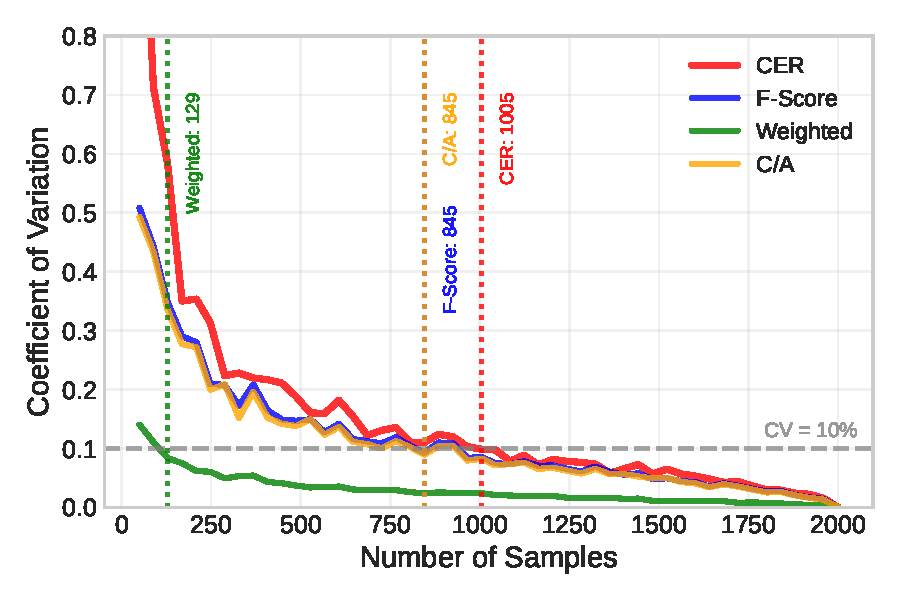
\includegraphics[width=\textwidth]{Figures/cv_comparison.pdf}
        \vspace{0.8em}
        \caption{Coefficient of variation of RI when evaluating on subsets of the full dataset. \cm{Add significance test}}
        \label{fig:refusal_index_cv_subset}
    \end{minipage}
    \hfill
    \begin{minipage}[t]{0.48\textwidth}
        \centering
        \vspace{-18.8em}
        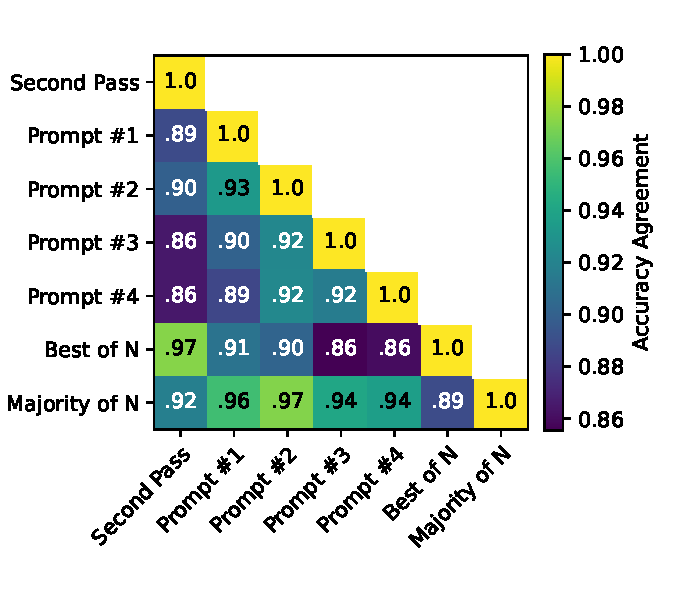
\includegraphics[width=\textwidth]{Figures/prompt_acc_agreement.pdf}
        \caption{Accuracy agreement between different prompt strategies.}
        \label{fig:prompt_acc_agreement}
    \end{minipage}
\end{figure}

We next examine how variations in prompt design affect the RI evaluation. Our experimental setup uses four distinct first-pass prompts, each with different few-shot examples and instructions, to induce varying refusal rates. For the second pass, a single, simpler prompt is used to compel the model to answer all previously refused questions. Although these prompts are designed to produce different refusal rates, it is crucial to verify that they do not introduce confounding effects on model accuracy, which would in turn impact the RI calculation.

To assess this, we measure the accuracy agreement between pairs of prompt strategies. Agreement is calculated as the proportion of questions for which both prompts yielded the same correctness label, considering only the questions answered by both. As shown in Figure~\ref{fig:prompt_acc_agreement}, the accuracy agreement between different first-pass prompts is consistently high (over 90\%). This indicates that the choice of prompt strategy does not significantly alter the model's underlying accuracy on the questions it chooses to answer. Furthermore, the high agreement involving the forced-answer (second-pass) prompt validates its use for effectively estimating the model's baseline accuracy ($\mu$).

\end{document}